\section{\SecAdvanceMapprojectionSetting} \label{sec:adv_mapproj}
%------------------------------------------------------
計算領域の位置と投影法は、設定ファイルの\verb|PARAM_MAPPROJ|の項目を編集することで設定できる。
\textcolor{red}{\bf この設定も、pp\_***.conf、init\_***.conf、run\_***.confの設定ファイルの間で
必ず一致させなければならない。}はじめに下記の例をもとに説明する。\\

\noindent {\small {\gt
\ovalbox{
\begin{tabularx}{140mm}{l}
\verb|&PARAM_MAPPROJ| \\
\verb| MPRJ_basepoint_lon = 138.727778D0,| \\
\verb| MPRJ_basepoint_lat = 35.360556D0,| \\
\verb| MPRJ_type          = 'MER',| \\
\verb|/| \\
\end{tabularx}
}}}\\

\noindent
まず\nmitem{MPRJ_basepoint_lat}と\nmitem{MPRJ_basepoint_lon}は、
計算領域の中心の緯度・経度を表す。
SCALE-RMでは、北緯を正、南緯を負の値として表現し、
経度は0度を起点に右回りで表現するため、
この設定では計算領域の
中心が北緯35.360556度、東経138.727778度に位置することになる。
この場所を中心に指定された大きさで、計算領域が
設定される
\footnote{デフォルトではメルカトル図法に基づいて緯度・経度を計算する際の基準とする緯度は、
\nmitem{MPRJ_basepoint_lat}の値が使用されるが、\nmitem{MPRJ\_M\_lat}を用いて
任意の緯度を指定することもできる。}。
実際にはSCALE-RM内部での格子点は、
実距離に基づいて格子点が配置される。
このため、設定された投影法では、実距離に基づいた緯度・経度座標が計算される。
この緯度・経度情報は、すべてのSCALEのNetCDF形式の出力ファイルに含まれている。

\nmitem{MPRJ_type}は、地図投影法の種類を表しており、\verb|MER|はメルカトル図法を意味する。
SCALEで現在選択できる地図投影法とその指定文字列は表\ref{tab:map_proj}のとおりである。

\begin{table}[tbh]
\begin{center}
\caption{SCALEで選択できる地図投影法}
\begin{tabularx}{150mm}{|l|X|} \hline
 \rowcolor[gray]{0.9} 地図投影法 & \verb|MPRJ_type| \\ \hline
 地図投影なし(理想実験用)& \verb|NONE| \\ \hline
 ランベルト正角円錐図法 & \verb|LC| \\ \hline
 極心平射図法(ポーラーステレオ) & \verb|PS| \\ \hline
 メルカトル図法 & \verb|MER| \\ \hline
 正距円筒図法 & \verb|EC| \\ \hline
\end{tabularx}
\label{tab:map_proj}
\end{center}
\end{table}

ここで、ランベルト正角円錐図法の設定方法については、設定方法が異なるため以下に説明する。
ここでは、現実大気実験チュートリアルで使用した\verb|run.conf|ファイルを例に挙げる。\\

\noindent {\small {\gt
\ovalbox{
\begin{tabularx}{140mm}{l}
\verb|&PARAM_MAPPROJ| \\
\verb| MPRJ_basepoint_lon = 135.220404D0,| \\
\verb| MPRJ_basepoint_lat = 34.653396D0,| \\
\verb| MPRJ_type          = 'LC',| \\
\verb| MPRJ_LC_lat1       =  30.00D0,| \\
\verb| MPRJ_LC_lat2       =  40.00D0,| \\
\verb|/| \\
\end{tabularx}
}}}\\

SCALE-RMでは2標準緯線型の実装を採用しているため、投影を決定する上で2つの標準緯線の
位置を指定する必要がある。2つの標準緯線に挟まれた領域では、
緯線・経線の長さの比が地球楕円体面上における
長さの比と近くなるように調節される。
従って、標準緯線を設定する
\nmitem{MPRJ_LC_lat1}と\nmitem{MPRJ_LC_lat2}の項目が追加されている。
それぞれ、南側、北側の標準緯線の値の単位は、degreeで指定する。

さらに下記のように\nmitem{MPRJ_basepoint_x}と\nmitem{MPRJ_basepoint_y}という変数を用いることで、
地図投影中心と計算領域中心をずらすこともできる。\\

\noindent {\small {\gt
\ovalbox{
\begin{tabularx}{140mm}{l}
\verb|&PARAM_MAPPROJ| \\
\verb| MPRJ_basepoint_lon = 135.220404D0,| \\
\verb| MPRJ_basepoint_lat = 34.653396D0,| \\
\verb| MPRJ_basepoint_x   = 100.0D0,| \\
\verb| MPRJ_basepoint_y   = 100.0D0,| \\
\verb| MPRJ_type          = 'LC',| \\
\verb| MPRJ_LC_lat1       =  30.00D0,| \\
\verb| MPRJ_LC_lat2       =  40.00D0,| \\
\verb|/| \\
\end{tabularx}
}}}\\

\noindent 
\nmitem{MPRJ_basepoint_x}と\nmitem{MPRJ_basepoint_y}は、地図投影中心の位置を、
計算領域の南西端(左下角)からの距離で指定するパラメータで、
単位はメートルである。
これらを指定しない場合は、デフォルト設定として計算領域中心と
地図投影中心の位置は一致する。
上記の場合とデフォルト設定の場合を比較したものを図\ref{fig:map_lc}に示す。
図\ref{fig:map_lc}aはデフォルト設定で投影中心と計算領域中心が一致している場合、
図\ref{fig:map_lc}bは、計算領域の位置を投影中心からずらした場合の関係を表している。
図\ref{fig:map_lc}bでは、計算領域の南西端から
\nmitem{MPRJ_basepoint_x}と\nmitem{MPRJ_basepoint_y}で指定した
距離だけ離れた位置に投影中心がある。

\begin{figure}[t]
\begin{center}
  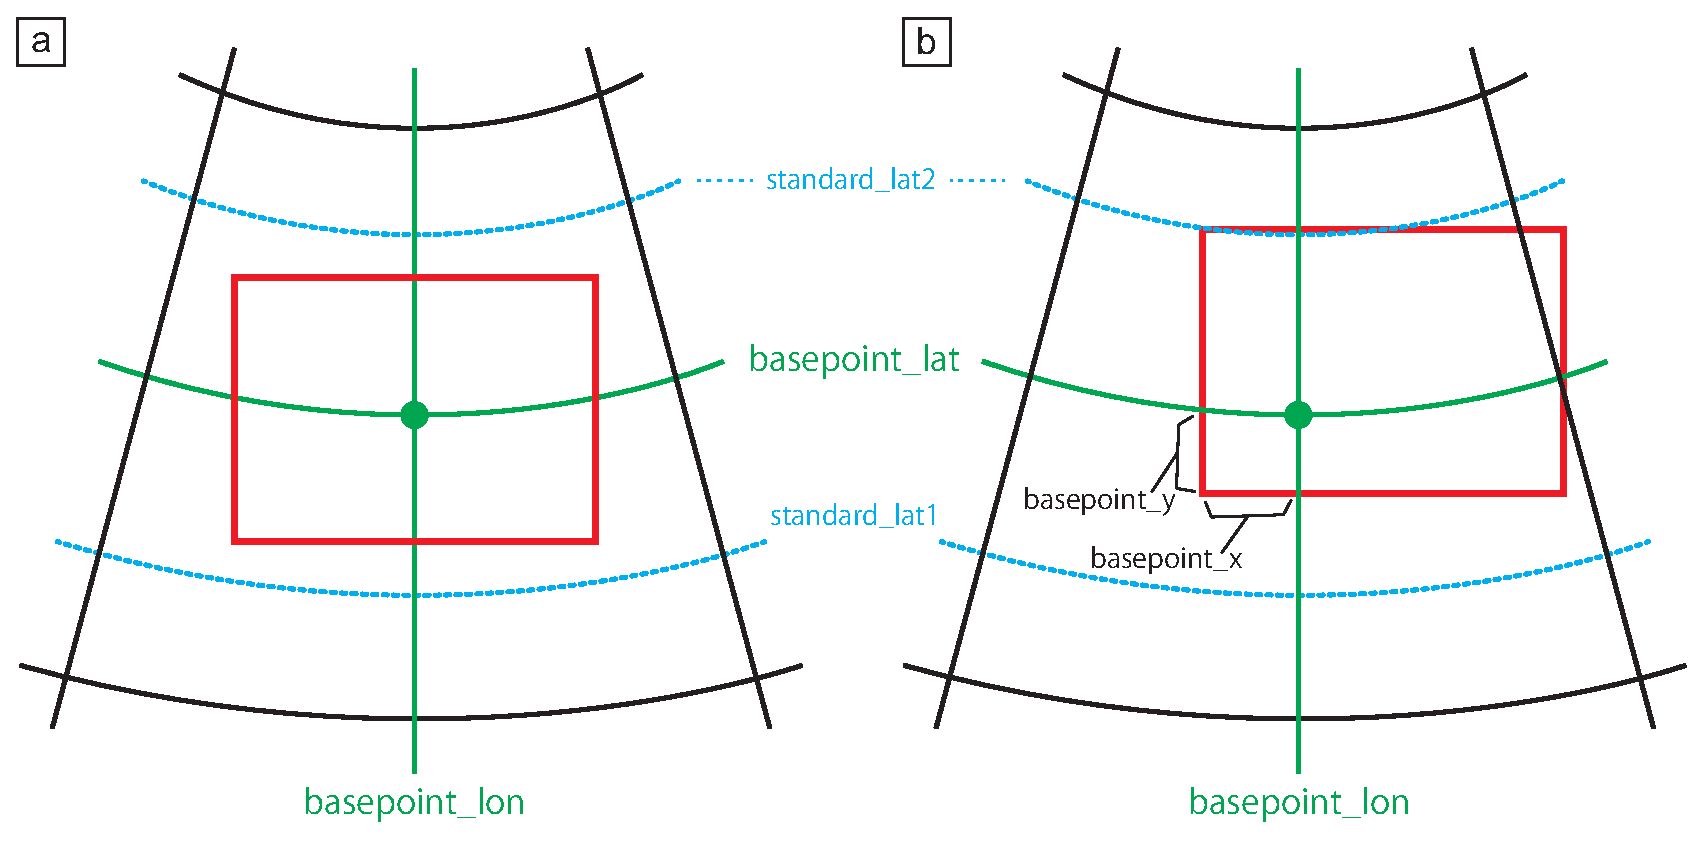
\includegraphics[width=0.8\hsize]{./figure/LC_latlon_xy.eps}\\
  \caption{投影中心と計算領域の関係:(a)はデフォルト設定の場合、(b)は計算領域の位置を投影中心からずらした場合。
  赤線の矩形が計算領域を表す。}
  \label{fig:map_lc}
\end{center}
\end{figure}

